\documentclass[10pt,a4paper,noendnumber=true]{scrartcl}
%german umlauts and localization
\usepackage[utf8]{inputenc} 
\usepackage[T1]{fontenc}
\usepackage[english]{babel}
\usepackage[dvipsnames]{xcolor}
\usepackage{booktabs}
\usepackage{tabularx}


\usepackage{geometry}
\geometry{
	a4paper,
	total={170mm,257mm},
	left=20mm,
	top=20mm,
}

\newcommand\pro{\item[$+$]}
\newcommand\con{\item[$-$]}

%figures etc.
\usepackage[pdftex]{graphicx}
\usepackage{standalone} %externalize files for faster compilation
\usepackage{float}

%mathematical symbols
\usepackage{latexsym} % special symbols 
\usepackage{amsmath,amssymb,amsthm}
\usepackage{textcomp} % supports the Text Companion fonts, 
\usepackage{mathrsfs}  % for script-like fonts in math mode
\usepackage{nicefrac} % nice fracs in text

%units
\usepackage{siunitx}
\DeclareSIUnit{\bar}{bar}
\sisetup{output-product=\ensuremath{\cdot},exponent-product=\ensuremath{\cdot}}

%tikz
\usepackage{tikz}
\usepackage{tikzscale}
\usepackage{pgfplots} 
\usepackage{pdflscape}
\usepackage[european]{circuitikz}
\pgfplotsset{compat=newest} 
\pgfplotsset{plot coordinates/math parser=false}
\usetikzlibrary{shapes.geometric}
\usetikzlibrary{arrows.meta}
\usetikzlibrary{arrows}
\usetikzlibrary{math}
\usetikzlibrary{shapes.symbols,shadows}

%bib stuff
\usepackage[draft = false]{hyperref}
\usepackage{csquotes}
\usepackage[backend=biber,style=ieee]{biblatex}
%\addbibresource{bib.bib}

%align multi pgfplots
\pgfplotsset{yticklabel style={text width=3em,align=right}}

\usetikzlibrary{external}
\tikzexternalize[optimize=false,prefix=tikz/] % activate!

\usepackage{subfig}
\setlength\parindent{0pt}

\begin{document}
\begin{titlepage}
\begin{sffamily}
\begin{center}
\begin{minipage}{1\textwidth}
      \begin{center} 
      
\includegraphics[height=0.4 \textwidth]{juas.jpeg} 
      \end{center} 
    \end{minipage}
\vspace{4.5cm}

\rule{\linewidth}{1.5pt} \\[0.5cm]
\Large \textbf{Magnet design for MedAustron} \\[0.5cm]
\rule{\linewidth}{1.5pt} \\
\vfill
\Large Group 3 : \\ [0.5cm]
\normalsize Gael Craviero, Sophie Morard, Marvin Noll, Abhishek Panchal, Katyayni Tiwari  \\ [0.5cm]
\normalsize 28 February 2022
\end{center}
\end{sffamily}
\end{titlepage}
\tableofcontents
\newpage
\section*{Introduction}
\addcontentsline{toc}{part}{Introduction}
The aim of this report is to present the analytical design and simulation of three bending magnets for MedAustron's medium energy beam transfer line.
\section{Analytical}
\subsection{Magnet type decision}
The arguments for and against a H-type magnet are:
\begin{itemize}
\pro Mechanically rigid
\pro Symmetrical
\pro Less iron than C-shape
\con Hard to get the beam pipe in and out
\end{itemize}

\subsection{Aperture Height}
The aperture height is given as the sum of the good field region $h_\text{GFR} = 2\cdot \text{GFR}_y$, the thickness of the vacuum pipe $d_\text{vacuum}$ and a tolerance for installation and thermal expansion $d_\text{tolerance}$ as
\begin{align}
    h &= h_\text{GFR} + 2\cdot d_\text{vacuum} + d_\text{tolerance} \\
      &= 2\cdot\SI{23}{\mm} + 2\cdot \SI{2}{\mm} + \SI{2}{\mm}\nonumber\\ 
      &= \SI{52}{\mm}. \nonumber
\end{align}

\subsection{Flux Density}
The total bending angle generated by all $m=3$ magnets is
\begin{equation}
    \theta_\text{tot} = 3 \cdot \theta_\text{mag} = 3 \cdot \SI{36}{\degree} = \SI{108}{\degree}.
\end{equation}

The magnetic length of the (dipole) magnet can be approximated by
\begin{align}
    l_\text{mag} &= l_\text{iron, max} + 2hk \\
    &= \SI{0.340}{\meter} + 2\cdot 0.55 \cdot \SI{52}{\mm}\nonumber\\
    &= \SI{397.2}{\mm}.\nonumber
\end{align}

With the definition of the radian ($\theta=\nicefrac{b}{\rho}$) and the arc length $b=l_\text{mag}$, the bending radius $\rho$ is

\begin{align}
    \theta_\text{mag} &= \frac{l_\text{mag}}{\rho} \\
    \Rightarrow \rho  &= \frac{l_{mag}}{2\cdot\sin(\theta_\text{mag}/2)}\\
    &= \frac{\SI{397.2}{\mm}}{2\cdot \sin(\SI{0.3141}{\radian})} \\
    &= \SI{0.642}{\meter}. \nonumber
\end{align}

With the given minimum and maximum $(B\rho)$ for a proton and a $C^{6+}$ beam, the minimum and maximum needed flux densities are
\begin{align}
    B_\text{min} &= \frac{(B \rho)_\text{min}}{\rho} = \frac{\SI{0.383}{\tesla\meter}}{\SI{0.642}{\meter}} = \SI{0.596}{\tesla}\\
    B_\text{max} &= \frac{(B \rho)_\text{max}}{\rho} = \frac{\SI{0.766}{\tesla\meter}}{\SI{0.642}{\meter}} = \SI{1.19}{\tesla}
\end{align}


\newpage
\subsection{Pole design and yoke dimensioning}
With the given field quality inside the GFR $\nicefrac{\Delta B}{B_0} = \num{1e-3}$,
the optimized normalized pole overhang is\footnote{Compared to the unoptimized $x_\text{unoptimized}= 1.5898$}
\begin{align}
    x_\text{optimized} &= 2\frac{a_\text{optimized}}{h} \\
    &= -0.14 \ln\left[\frac{\Delta B}{B_0}\right] -0.25 \nonumber\\
    &= 0.7171. \nonumber
\end{align}

This equals a pole overhang of
\begin{align}
    a_\text{optimized} &= \frac{h\cdot x_\text{optimized}}{2} \\
    &= \frac{\SI{52}{\mm} \cdot 0.7171}{2} \nonumber\\
    &= \SI{18.645}{\mm}.\nonumber
\end{align}

With taking the sagitta
\begin{equation}
    s= \rho\left(1-\cos \nicefrac{\theta}{2}\right)
    = \SI{31.42}{\mm} 
\end{equation}
into account, the the pole width $w$ computes to
\begin{align}
	w & =  2 \left(\text{GFRx} + a_\text{optimized}\right) +  \rho\left(1-\cos \nicefrac{\theta}{2}\right)          \\
	  & =  2 \left(\SI{20}{\mm} + \SI{18.645}{\mm}\right) + \SI{31.42}{\mm}\nonumber \\
	  & = \SI{108.71}{\mm}. \nonumber
\end{align}

The yoke thickness $w_\text{leg}$ is ($B_\text{max} = \SI{1.19}{\tesla}$, $w = \SI{108.71}{\mm}$, $h = \SI{52}{\mm}$, $B_\text{saturation} = \SI{1.4}{\tesla}$)
\begin{align}
w_\text{leg} &= B_\text{max} \cdot \frac{w + 2 \cdot h}{2 \cdot B_\text{saturation}} \\
&\simeq \SI{90.4}{\mm}
\end{align}


\subsection{Excitation Current}
The ampereturns are computed as
\begin{align}
    (NI)_\text{dipole, min} &= \frac{B_\text{min}\,h}{2\,\mu_0} = \frac{\SI{0.596}{\tesla} \cdot \SI{52}{\mm}}{2\cdot \mu_0} = \SI{12.331}{\kilo\ampere}\\
    (NI)_\text{dipole, max} &= \frac{B_\text{max}\,h}{2\,\mu_0} = \frac{\SI{1.19}{\tesla} \cdot \SI{52}{\mm}}{2\cdot \mu_0} = \SI{24.621}{\kilo\ampere}
\end{align}

\begin{figure}[H]
\centering
\includegraphics[width=0.5\textwidth]{img/winding.tikz}
\caption{Cross section of the copper winding showing  insulation(\textcolor{orange}{$\blacksquare$}) and water channel(\textcolor{blue!20}{$\blacksquare$})}
\label{fig:winding}
\end{figure}

With the given dimensions of the copper winding (see \autoref{fig:winding}) and using 
\begin{align}
A_\text{rounded edges} &= 4 \cdot  A_\text{rounded edge} = 4 \frac{r_o^2 (4-\pi)}{4} = r_o^2(4-\pi) \\
A_\text{water channel} &= \pi r_c^2
\end{align}

the copper cross section area is
\begin{align}
	A_\text{copper} & = a^2 - \underbrace{r_o^2(4-\pi)}_{A_\text{rounded edges}} - \underbrace{\pi r_c^2}_{A_\text{water channel}} \\
	  & = \SI{121}{\mm\squared} - \SI{0.8584}{\mm\squared} - \SI{28.274}{\mm\squared} \nonumber                      \\
	  & = \SI{91.867}{\mm\squared} \nonumber
\end{align}

With the given maximum current density of $j_\text{max}=\SI{6}{\ampere\per\mm\squared}$, the maximum possible current in the winding is
\begin{align}
I_\text{max} &= j_\text{max} \cdot A_\text{copper} \\
 &=\SI{6}{\ampere\per\mm\squared} \cdot \SI{91.867}{\mm\squared} \nonumber\\ 
 &= \SI{551.202}{\ampere}. \nonumber
\end{align}

With the calculated ampereturns, the necessary minimum number of turns are then
\begin{align}
    N_{B_\text{min}} &= \left\lceil\frac{(NI)_\text{min}}{I_\text{max}}\right\rceil = 23\\
    N_{B_\text{max}} &= \left\lceil\frac{(NI)_\text{max}}{I_\text{max}}\right\rceil = 45
\end{align}

As it is easier to lower the current then to change the number of turns, the minimum number of turns should be $N_{B_\text{max}}$.

To full fill the empirical good practice $\nicefrac{N_\text{horizontal}}{N_\text{vertical}}=2$, the number of turn is set to
\begin{equation}
    N=N_\text{horizontal} \times N_\text{vertical} = 10 \times 5 = 50.
\end{equation}

With the new $N=50$, the winding current is
\begin{equation}
    I = \frac{(NI)_\text{max}}{50} = \SI{492.42}{\ampere},
\end{equation}
which is well below the maximum current of the power supply ($I_\text{max}=\SI{600}{\ampere}$).

\subsection{Coil Parameters}
The coil width and height are given by (see \autoref{fig:coil})
\begin{equation}
    w_\text{coil}=N_\text{horizontal} \cdot (a+d_\text{insulation}) + 2\cdot(d_\text{epoxy} + d_\text{air}) = \SI{128}{\mm}
\end{equation}
and
\begin{equation}
    h_\text{coil}=N_\text{vertical} \cdot (a+d_\text{insulation}) + 2\cdot(d_\text{epoxy} + d_\text{air}) = \SI{68}{\mm}
\end{equation}
using $N_\text{horizontal}=10$, $N_\text{vertical}=5$, $a=\SI{11}{\mm}$, $d_\text{insulation}=\SI{1}{\mm}$, $d_\text{epoxy}=\SI{2}{\mm}$ and $d_\text{air}=\SI{2}{\mm}$.

\begin{figure}[H]
\centering
\includegraphics[width=\textwidth]{img/coil.tikz}
\caption{Cross section of one coil showing copper(\textcolor{black}{$\square$}), insulation(\textcolor{orange}{$\blacksquare$}), 
the water channels(\textcolor{blue!30}{$\blacksquare$}),
the coil epoxy coating(\textcolor{red!30}{$\blacksquare$}) and
the air gap around the coil(\textcolor{green!30}{$\blacksquare$})}
\label{fig:coil}
\end{figure}

With the pole perimeter
\begin{equation}
	p = 2 \cdot l_\text{iron} + 2 \cdot w = \SI{897}{\mm},
\end{equation}
the average turn length is ($l_\text{iron} = \SI{340}{\mm}$, $w = \SI{109}{\mm}$ and $w_\text{coil} = \SI{128}{\mm}$)
\begin{equation}
    l_\text{avg}= p + 4 \cdot w_\text{coil} = \SI{1409}{\mm}.
\end{equation}

The resistance of one coil winding is (with $1/\sigma_\text{Cu}=\SI{1.72}{\micro\ohm\cm}$)
\begin{align}
R_c&=\frac{N\cdot l_\text{avg}}{A\cdot\sigma_\text{Cu}} \\
&= \frac{50 \cdot \SI{1409}{\mm}}{\SI{91.867}{\mm\squared}\cdot \nicefrac{1}{\SI{1.72}{\micro\ohm\cm}}} \nonumber\\
&= \SI{13.19}{\milli\ohm} \nonumber
\end{align}

With the number of coils per magnet $m$, the DC steady-state voltage per magnet is
\begin{align}
V_m &= I \cdot m\,R_c \\
&= \SI{492.42}{\ampere} \cdot 2 \cdot \SI{13.19}{m\ohm} \nonumber\\
&= \SI{12.99}{\volt}.\nonumber
\end{align}

The total voltage over all magnets is (number of magnets $M$)
\begin{align}
V_\text{total} &= M \cdot V_m \\
&= 3 \cdot \SI{12.99}{\volt} \nonumber\\
&= \SI{38.97}{\volt}.\nonumber
\end{align}
This is well below the maximum output voltage of the power supply ($V_\text{total, max}=\SI{80}{\volt}$).

The dissipated power in one magnet is calculated to
\begin{align}
P_m &= V_m \cdot I = I^2 \cdot m\,R_c \\
&= \SI{13.19}{\volt} \cdot \SI{492.42}{\ampere} \nonumber\\
&= \SI{6.495}{\kilo\watt}.\nonumber
\end{align}

\subsection{Cooling}
With the given $\Delta T=\SI{15}{\kelvin}$ and the dissipated power $P_m=\SI{6.495}{\kilo\watt}$, the total required water flow in one magnet is
\begin{equation}
    Q = 14.3 \frac{P_m}{\Delta T} \cdot \num{1e-3} = \SI{6.19}{\liter\per\minute}
\end{equation}

Using the length of cooling circuit for one coil is ($K_c=1$ and $K_w=1$)
\begin{align}
    l &= \frac{K_c\,N\,l_\text{avg}}{K_w} \\
    &= \frac{1\cdot50\cdot\SI{1409}{\mm}}{1} \nonumber\\ 
    &= \SI{70.5}{\meter}. \nonumber
\end{align}

The pressure drop over a cooling circuit is given by ($d=2r_c=\SI{6}{\mm}$)
\begin{equation}
    \Delta p = 60 \cdot l \cdot \frac{Q^{1.75}}{d^{4.75}} 
\end{equation}

This can be interpreted a (non-linear) hydraulic equivalent to Ohm's law in the electrical domain:
\begin{equation}
	\Delta p = \underbrace{\frac{60 \cdot l}{d^{4.75}}}_R \cdot Q^{1.75} = R \cdot Q^{1.75}
\end{equation}

The hydraulic resistance of one coil is given (in AU) as
\begin{equation}
R= \frac{60 \cdot l}{d^{4.75}} = 0.85
\end{equation}

To cool one magnet, the cooling circuits can either be connected in series or in parallel (see \autoref{fig:cool}).

\begin{figure}[H]
	\centering\setcounter{subfigure}{0}
	\subfloat[Series connection]{\includegraphics[width=0.8\textwidth]{img/coolingSeries.tikz}}\\
	\subfloat[Parallel connection]{\includegraphics[width=0.8\textwidth]{img/coolingParallel.tikz}}
	\caption{Possible cooling circuit configurations}\label{fig:cool}
\end{figure}

For both cases, the pressure drops are
\begin{align}
\Delta p_\text{Series} &= 2 \cdot 0.85 \cdot 6.2^{1.75} = \SI{41.4}{\bar} \\
\Delta p_\text{Parallel} &= 0.85 \cdot 3.1^{1.75} = \SI{6.2}{\bar}
\end{align}

As the series connection pressure drop exceeds the limit of the pump ($\Delta p_\text{max}=\SI{7}{\bar}$), the parallel connection is used.

The average flow velocity in this case is
\begin{equation}
    u_\text{avg} = 16.67 \cdot \frac{Q}{A} = 16.67 \cdot \frac{4\cdot Q}{\pi d^2} = 16.67 \cdot \frac{4 \cdot \SI{3.1}{\liter\per\minute}}{\pi \cdot (\SI{6}{\mm})^{2}} = \SI{1.827}{\meter\per\second}.
\end{equation}

Reynolds number (with $v=\SI{6.58e-7}{\meter\squared\per\second}$) is computed as
\begin{equation}
    R_e = d \cdot \frac{u_\text{avg}}{v} \cdot \num{1e-3} = \num{16660}.
\end{equation}
From $R_e>4000$ turbulent flow can be assumed for the flow in the water channels, which is needed for equal heat distribution.



\newpage
\section{Numerical}

\begin{figure}[H]
\centering
\includegraphics[width=\textwidth]{img/quaterH.tikz}
\caption{Input data for numerical simulation; all measurements in \si{\mm}; drawing not to scale}
\label{data}
\end{figure}

\begin{table}[H]
\centering
\caption{Relevant magnet parameters}
\begin{tabular}{ll}
\toprule
Name & Value \\
\midrule
Flux density $B$ & \SIrange{0.596}{1.19}{\tesla}\\
Gap height $h$ & \SI{52}{\mm}\\
Pole width $w$ & \SI{110}{\mm}\\
Ampereturns $NI$ & \SIrange{12.3}{24.6}{\kilo\ampere}\\
\bottomrule
\end{tabular}
\end{table}
By using the data of \autoref{data} on FEMM, the current $I = \SI{492.42}{\ampere}$ and the number of turns $N = 50$, the result of the simulation obtained is shown in \autoref{FEMM1}.
The simulation area is set to $600 \times 400$. This way the simulated region is much bigger than the magnet and there is not cut-off of significant percentages of the field lines.

\begin{figure}[H]
    \centering
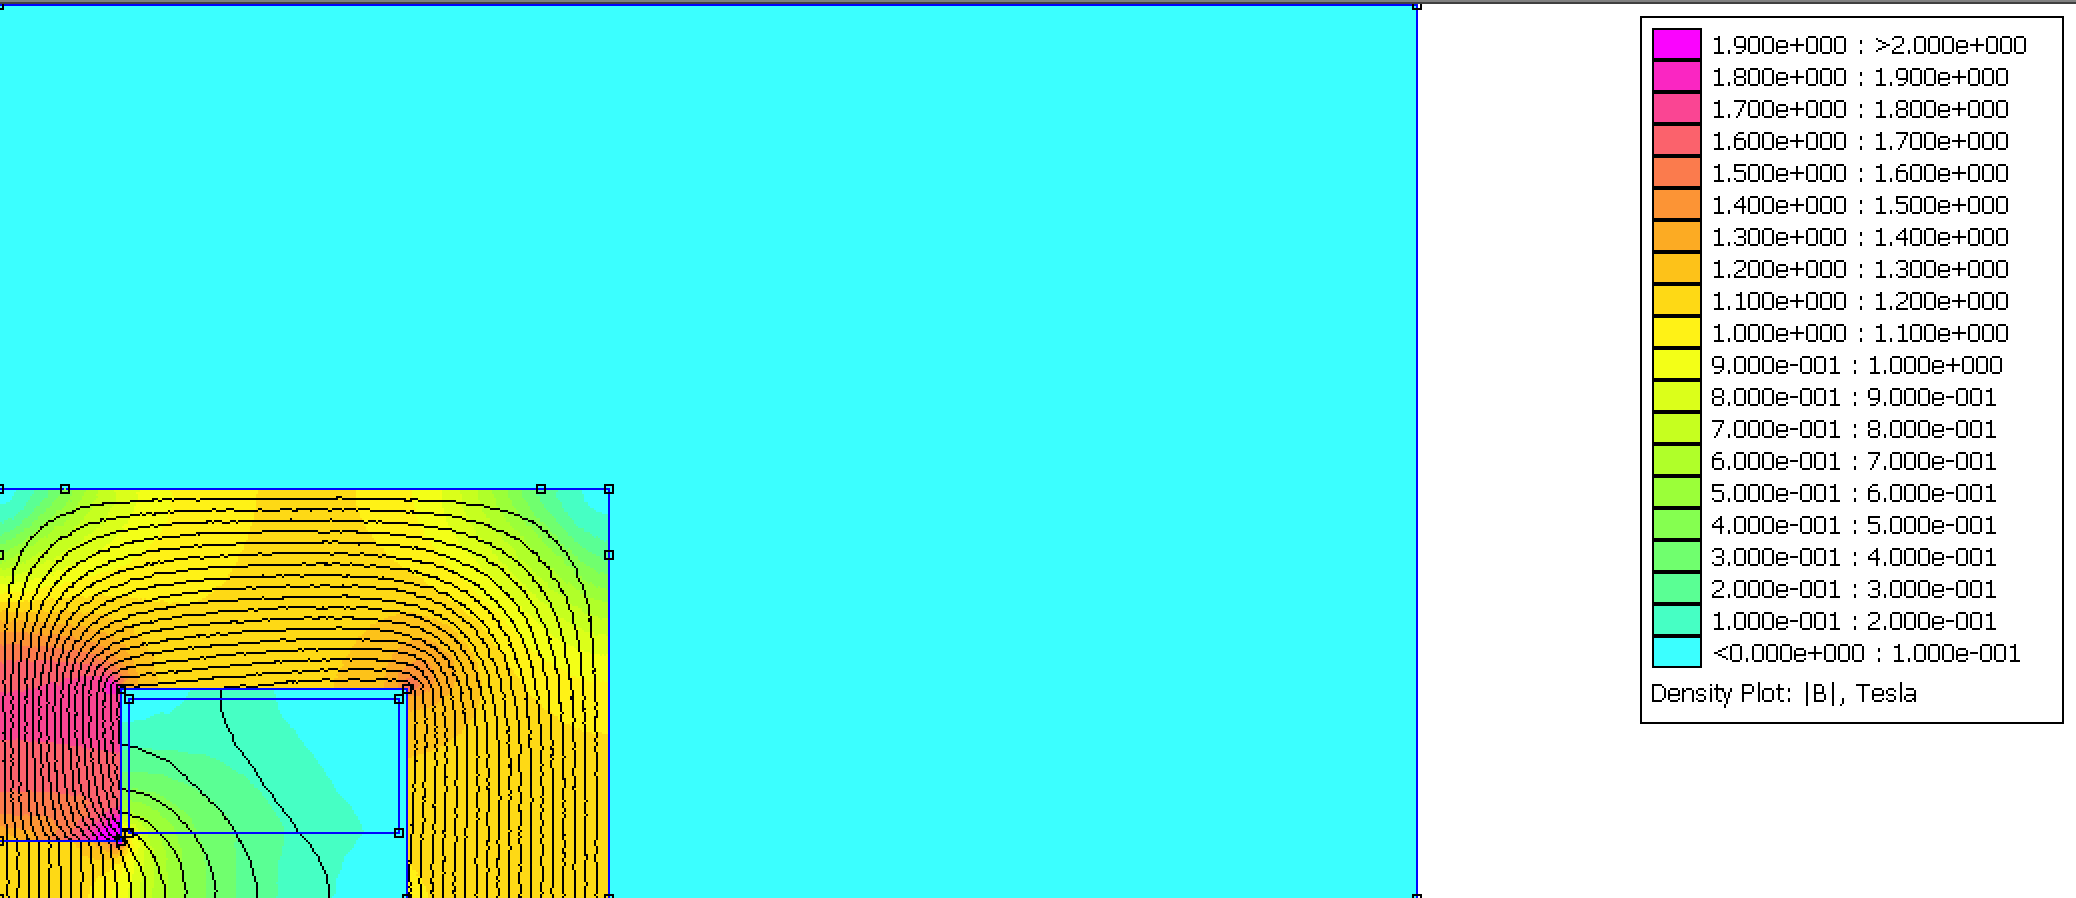
\includegraphics[width=1 \textwidth]{magnet_non_OP.png} 
\caption{Result of FEMM for the magnet with the initial data}
\label{FEMM1}
\end{figure} 

At the pole level, the value of the $B$ field can be over \SI{2}{\tesla} in the yoke, there is a lot of saturation. Therefore, the magnet needs to be optimized.
For this, the pole width is not modified but instead, the upper part of the pole is widened to \SI{90}{\mm}, like the value of the pole thickness that was calculated to optimized the field quality. Also the region of the yoke, where the field is very weak, is cut. The result of this simulation is shown in \autoref{FEMM2}.

\begin{figure}[H]
    \centering
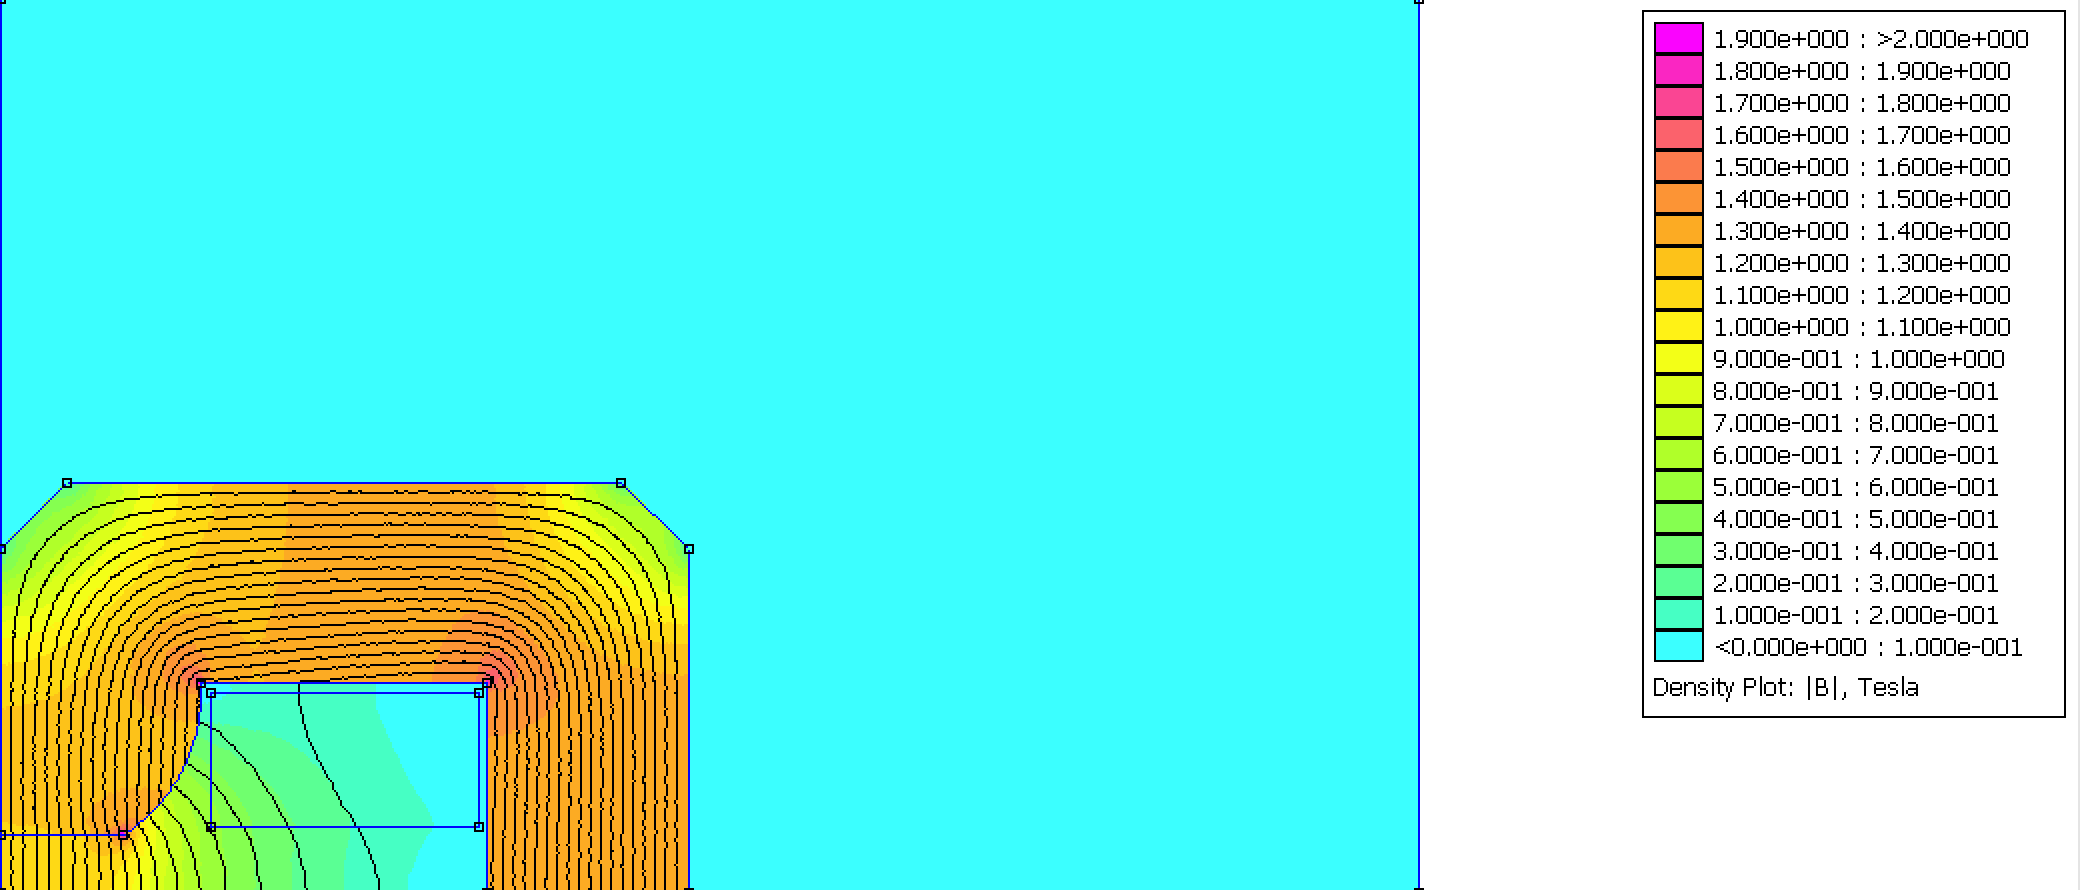
\includegraphics[width=1 \textwidth]{magnet_OP.png} 
\caption{Result of FEMM for the modified magnet for optimization}
\label{FEMM2}
\end{figure} 

The saturation has been definitely reduced and the field in the center part is homogeneous and around \SI{1.2}{\tesla}. The left part of the yoke has been rounded off for the upper part of the pole to widen more rapidly and to optimize the good field region. To have more straight field lines in the center of the magnet the rounded part could maybe be done as staircase.

\end{document}

